% Options for packages loaded elsewhere
\PassOptionsToPackage{unicode}{hyperref}
\PassOptionsToPackage{hyphens}{url}
%
\documentclass[
]{article}
\usepackage{amsmath,amssymb}
\usepackage{iftex}
\ifPDFTeX
  \usepackage[T1]{fontenc}
  \usepackage[utf8]{inputenc}
  \usepackage{textcomp} % provide euro and other symbols
\else % if luatex or xetex
  \usepackage{unicode-math} % this also loads fontspec
  \defaultfontfeatures{Scale=MatchLowercase}
  \defaultfontfeatures[\rmfamily]{Ligatures=TeX,Scale=1}
\fi
\usepackage{lmodern}
\ifPDFTeX\else
  % xetex/luatex font selection
\fi
% Use upquote if available, for straight quotes in verbatim environments
\IfFileExists{upquote.sty}{\usepackage{upquote}}{}
\IfFileExists{microtype.sty}{% use microtype if available
  \usepackage[]{microtype}
  \UseMicrotypeSet[protrusion]{basicmath} % disable protrusion for tt fonts
}{}
\makeatletter
\@ifundefined{KOMAClassName}{% if non-KOMA class
  \IfFileExists{parskip.sty}{%
    \usepackage{parskip}
  }{% else
    \setlength{\parindent}{0pt}
    \setlength{\parskip}{6pt plus 2pt minus 1pt}}
}{% if KOMA class
  \KOMAoptions{parskip=half}}
\makeatother
\usepackage{xcolor}
\usepackage[margin=1in]{geometry}
\usepackage{color}
\usepackage{fancyvrb}
\newcommand{\VerbBar}{|}
\newcommand{\VERB}{\Verb[commandchars=\\\{\}]}
\DefineVerbatimEnvironment{Highlighting}{Verbatim}{commandchars=\\\{\}}
% Add ',fontsize=\small' for more characters per line
\usepackage{framed}
\definecolor{shadecolor}{RGB}{248,248,248}
\newenvironment{Shaded}{\begin{snugshade}}{\end{snugshade}}
\newcommand{\AlertTok}[1]{\textcolor[rgb]{0.94,0.16,0.16}{#1}}
\newcommand{\AnnotationTok}[1]{\textcolor[rgb]{0.56,0.35,0.01}{\textbf{\textit{#1}}}}
\newcommand{\AttributeTok}[1]{\textcolor[rgb]{0.13,0.29,0.53}{#1}}
\newcommand{\BaseNTok}[1]{\textcolor[rgb]{0.00,0.00,0.81}{#1}}
\newcommand{\BuiltInTok}[1]{#1}
\newcommand{\CharTok}[1]{\textcolor[rgb]{0.31,0.60,0.02}{#1}}
\newcommand{\CommentTok}[1]{\textcolor[rgb]{0.56,0.35,0.01}{\textit{#1}}}
\newcommand{\CommentVarTok}[1]{\textcolor[rgb]{0.56,0.35,0.01}{\textbf{\textit{#1}}}}
\newcommand{\ConstantTok}[1]{\textcolor[rgb]{0.56,0.35,0.01}{#1}}
\newcommand{\ControlFlowTok}[1]{\textcolor[rgb]{0.13,0.29,0.53}{\textbf{#1}}}
\newcommand{\DataTypeTok}[1]{\textcolor[rgb]{0.13,0.29,0.53}{#1}}
\newcommand{\DecValTok}[1]{\textcolor[rgb]{0.00,0.00,0.81}{#1}}
\newcommand{\DocumentationTok}[1]{\textcolor[rgb]{0.56,0.35,0.01}{\textbf{\textit{#1}}}}
\newcommand{\ErrorTok}[1]{\textcolor[rgb]{0.64,0.00,0.00}{\textbf{#1}}}
\newcommand{\ExtensionTok}[1]{#1}
\newcommand{\FloatTok}[1]{\textcolor[rgb]{0.00,0.00,0.81}{#1}}
\newcommand{\FunctionTok}[1]{\textcolor[rgb]{0.13,0.29,0.53}{\textbf{#1}}}
\newcommand{\ImportTok}[1]{#1}
\newcommand{\InformationTok}[1]{\textcolor[rgb]{0.56,0.35,0.01}{\textbf{\textit{#1}}}}
\newcommand{\KeywordTok}[1]{\textcolor[rgb]{0.13,0.29,0.53}{\textbf{#1}}}
\newcommand{\NormalTok}[1]{#1}
\newcommand{\OperatorTok}[1]{\textcolor[rgb]{0.81,0.36,0.00}{\textbf{#1}}}
\newcommand{\OtherTok}[1]{\textcolor[rgb]{0.56,0.35,0.01}{#1}}
\newcommand{\PreprocessorTok}[1]{\textcolor[rgb]{0.56,0.35,0.01}{\textit{#1}}}
\newcommand{\RegionMarkerTok}[1]{#1}
\newcommand{\SpecialCharTok}[1]{\textcolor[rgb]{0.81,0.36,0.00}{\textbf{#1}}}
\newcommand{\SpecialStringTok}[1]{\textcolor[rgb]{0.31,0.60,0.02}{#1}}
\newcommand{\StringTok}[1]{\textcolor[rgb]{0.31,0.60,0.02}{#1}}
\newcommand{\VariableTok}[1]{\textcolor[rgb]{0.00,0.00,0.00}{#1}}
\newcommand{\VerbatimStringTok}[1]{\textcolor[rgb]{0.31,0.60,0.02}{#1}}
\newcommand{\WarningTok}[1]{\textcolor[rgb]{0.56,0.35,0.01}{\textbf{\textit{#1}}}}
\usepackage{graphicx}
\makeatletter
\def\maxwidth{\ifdim\Gin@nat@width>\linewidth\linewidth\else\Gin@nat@width\fi}
\def\maxheight{\ifdim\Gin@nat@height>\textheight\textheight\else\Gin@nat@height\fi}
\makeatother
% Scale images if necessary, so that they will not overflow the page
% margins by default, and it is still possible to overwrite the defaults
% using explicit options in \includegraphics[width, height, ...]{}
\setkeys{Gin}{width=\maxwidth,height=\maxheight,keepaspectratio}
% Set default figure placement to htbp
\makeatletter
\def\fps@figure{htbp}
\makeatother
\setlength{\emergencystretch}{3em} % prevent overfull lines
\providecommand{\tightlist}{%
  \setlength{\itemsep}{0pt}\setlength{\parskip}{0pt}}
\setcounter{secnumdepth}{-\maxdimen} % remove section numbering
\ifLuaTeX
  \usepackage{selnolig}  % disable illegal ligatures
\fi
\IfFileExists{bookmark.sty}{\usepackage{bookmark}}{\usepackage{hyperref}}
\IfFileExists{xurl.sty}{\usepackage{xurl}}{} % add URL line breaks if available
\urlstyle{same}
\hypersetup{
  pdftitle={Tutorial\_2.Rmd},
  pdfauthor={Amelia Mesich},
  hidelinks,
  pdfcreator={LaTeX via pandoc}}

\title{Tutorial\_2.Rmd}
\author{Amelia Mesich}
\date{2025-08-11}

\begin{document}
\maketitle

\hypertarget{packages-we-will-use}{%
\subsection{Packages we will use}\label{packages-we-will-use}}

Packages are collections of useful functions, data and documentation
written by other people as an extension of basic R features.

\begin{Shaded}
\begin{Highlighting}[]
\CommentTok{\# a collection of R packages including ggplot, lubridate, forcats, stringr, tidyr, dplyr}
\FunctionTok{library}\NormalTok{(tidyverse)}
\end{Highlighting}
\end{Shaded}

\begin{verbatim}
## Warning: package 'tidyverse' was built under R version 4.3.3
\end{verbatim}

\begin{verbatim}
## Warning: package 'ggplot2' was built under R version 4.3.3
\end{verbatim}

\begin{verbatim}
## Warning: package 'tibble' was built under R version 4.3.2
\end{verbatim}

\begin{verbatim}
## Warning: package 'readr' was built under R version 4.3.3
\end{verbatim}

\begin{verbatim}
## Warning: package 'purrr' was built under R version 4.3.2
\end{verbatim}

\begin{verbatim}
## Warning: package 'dplyr' was built under R version 4.3.2
\end{verbatim}

\begin{verbatim}
## Warning: package 'stringr' was built under R version 4.3.2
\end{verbatim}

\begin{verbatim}
## Warning: package 'forcats' was built under R version 4.3.3
\end{verbatim}

\begin{verbatim}
## Warning: package 'lubridate' was built under R version 4.3.3
\end{verbatim}

\begin{verbatim}
## -- Attaching core tidyverse packages ------------------------ tidyverse 2.0.0 --
## v dplyr     1.1.4     v readr     2.1.5
## v forcats   1.0.0     v stringr   1.5.1
## v ggplot2   3.5.1     v tibble    3.2.1
## v lubridate 1.9.3     v tidyr     1.3.1
## v purrr     1.0.2     
## -- Conflicts ------------------------------------------ tidyverse_conflicts() --
## x dplyr::filter() masks stats::filter()
## x dplyr::lag()    masks stats::lag()
## i Use the conflicted package (<http://conflicted.r-lib.org/>) to force all conflicts to become errors
\end{verbatim}

\begin{Shaded}
\begin{Highlighting}[]
\CommentTok{\#additional package that sets the working directory}
\FunctionTok{library}\NormalTok{(here)}
\end{Highlighting}
\end{Shaded}

\begin{verbatim}
## Warning: package 'here' was built under R version 4.3.2
\end{verbatim}

\begin{verbatim}
## here() starts at C:/Users/ameli/OneDrive/Documents/CSB-345-tutorials
\end{verbatim}

\begin{Shaded}
\begin{Highlighting}[]
\CommentTok{\#additional package to change the scales on a time series plot}
\FunctionTok{library}\NormalTok{(scales)}
\end{Highlighting}
\end{Shaded}

\begin{verbatim}
## Warning: package 'scales' was built under R version 4.3.2
\end{verbatim}

\begin{verbatim}
## 
## Attaching package: 'scales'
## 
## The following object is masked from 'package:purrr':
## 
##     discard
## 
## The following object is masked from 'package:readr':
## 
##     col_factor
\end{verbatim}

\#\#Section 1: Loading in the dataset

We will load in the data from the Bitsikas et al paper into a variable
called fish\_df. This is a subset of the total data and contains all the
observations from the month of August.

\begin{Shaded}
\begin{Highlighting}[]
\NormalTok{fish\_df }\OtherTok{\textless{}{-}} \FunctionTok{read.csv}\NormalTok{(}\AttributeTok{file =} \FunctionTok{here}\NormalTok{(}\StringTok{"zebrafish\_behaviour\_subset.csv"}\NormalTok{))}
\CommentTok{\#examine how the data is structured}
\FunctionTok{str}\NormalTok{(fish\_df)}
\end{Highlighting}
\end{Shaded}

\begin{verbatim}
## 'data.frame':    869486 obs. of  5 variables:
##  $ time    : chr  "2022-08-09 10:25:30" "2022-08-09 10:25:36" "2022-08-09 10:25:42" "2022-08-09 10:25:48" ...
##  $ Dist_6s : num  0.433 0.387 0.477 0.326 0.239 ...
##  $ genotype: chr  "WT" "WT" "WT" "WT" ...
##  $ daytime : chr  "day" "day" "day" "day" ...
##  $ state   : chr  "Wake" "Wake" "Wake" "Wake" ...
\end{verbatim}

We can see that this is a dataframe that contains the 869, 486
observations or rows.

Each observation has a timepoint (time column), the distance travelled
in 6 seconds (Dist\_6s column), the genotype of the individual (genotype
column), if the observation occured at day or night (daytime column) and
the sleep-wake state of the individual (state column).

\begin{Shaded}
\begin{Highlighting}[]
\CommentTok{\#look at the first 6 rows}
\FunctionTok{head}\NormalTok{(fish\_df)}
\end{Highlighting}
\end{Shaded}

\begin{verbatim}
##                  time   Dist_6s genotype daytime state
## 1 2022-08-09 10:25:30 0.4327311       WT     day  Wake
## 2 2022-08-09 10:25:36 0.3873116       WT     day  Wake
## 3 2022-08-09 10:25:42 0.4768259       WT     day  Wake
## 4 2022-08-09 10:25:48 0.3259950       WT     day  Wake
## 5 2022-08-09 10:25:54 0.2390276       WT     day  Wake
## 6 2022-08-09 10:26:00 0.3167992       WT     day  Wake
\end{verbatim}

\begin{Shaded}
\begin{Highlighting}[]
\CommentTok{\#open the full dataframe in a new tab}
\FunctionTok{View}\NormalTok{(fish\_df)}
\end{Highlighting}
\end{Shaded}

\hypertarget{section-2-convert-format-of-date-time-column}{%
\subsection{Section 2: Convert format of date-time
column}\label{section-2-convert-format-of-date-time-column}}

We will convert the time column to a date-time object using the function
as\_datetime() from lubridate.

We can also use the day(), hour() and minute() functions to extract the
day, hour and minute from the time.

\begin{Shaded}
\begin{Highlighting}[]
\NormalTok{fish\_df}\SpecialCharTok{$}\NormalTok{time }\OtherTok{\textless{}{-}} \FunctionTok{as\_datetime}\NormalTok{(fish\_df}\SpecialCharTok{$}\NormalTok{time)}
\NormalTok{fish\_df}\SpecialCharTok{$}\NormalTok{day }\OtherTok{\textless{}{-}} \FunctionTok{day}\NormalTok{(fish\_df}\SpecialCharTok{$}\NormalTok{time)}
\NormalTok{fish\_df}\SpecialCharTok{$}\NormalTok{hour }\OtherTok{\textless{}{-}} \FunctionTok{hour}\NormalTok{(fish\_df}\SpecialCharTok{$}\NormalTok{time)}
\NormalTok{fish\_df}\SpecialCharTok{$}\NormalTok{minute }\OtherTok{\textless{}{-}} \FunctionTok{minute}\NormalTok{(fish\_df}\SpecialCharTok{$}\NormalTok{time)}
\CommentTok{\#fish\_df$second \textless{}{-} second(fish\_df$time)}
\CommentTok{\#fish\_df$timestamp \textless{}{-} paste(fish\_df$hour, fish\_df$minute, fish\_df$second, sep = ":")}
\end{Highlighting}
\end{Shaded}

For the first plot, we will filter for just the wildtype (WT) data using
the filter() function. We will call the subset dataframe fish\_WT. This
subsets the dataframe from 869,486 rows to 263,682 rows.

\begin{Shaded}
\begin{Highlighting}[]
\NormalTok{fish\_WT }\OtherTok{\textless{}{-}} \FunctionTok{filter}\NormalTok{(fish\_df, genotype }\SpecialCharTok{==} \StringTok{"WT"}\NormalTok{)}
\end{Highlighting}
\end{Shaded}

\hypertarget{section-3-plotting-the-time-series}{%
\subsection{Section 3: Plotting the time
series}\label{section-3-plotting-the-time-series}}

The function ggplot allows us to create a customizable data
visualizations It requires the data to plot as the first variable, and
the aesthetics to be used when making the plot (typically this is the x
and y coordinates). You can then specify the type of plot you want to
make with additional mapping layers. Here we use geom\_line() but we
will go through other examples of plots supported by ggplot.

\begin{Shaded}
\begin{Highlighting}[]
\CommentTok{\#plot the raw observations (264k observations) from fish\_WT}
\CommentTok{\#set the x axis to be time and the y axis to be distance moved in 6s}
\FunctionTok{ggplot}\NormalTok{(}\AttributeTok{data =}\NormalTok{ fish\_WT, }\AttributeTok{mapping =} \FunctionTok{aes}\NormalTok{(}\AttributeTok{x =}\NormalTok{ time, }\AttributeTok{y =}\NormalTok{ Dist\_6s)) }\SpecialCharTok{+} \FunctionTok{geom\_line}\NormalTok{() }\SpecialCharTok{+} \FunctionTok{ggtitle}\NormalTok{(}\StringTok{"Plot 1: Zerbafish time series over 4 days"}\NormalTok{)}
\end{Highlighting}
\end{Shaded}

\includegraphics{Tutorial_2_files/figure-latex/Section 3.1-1.pdf}

We can look at the data from one day of observations. By using the pipe
operator \%\textgreater\% we can run this in one line. The pipe operator
takes the output of one function and passes it to be the input of a
second function and so on. First we pass the fish\_WT dataframe to the
filter() function and then pass the result of this (the filtered
dataframe) to ggplot and create the same time series plot as above.

\begin{Shaded}
\begin{Highlighting}[]
\CommentTok{\#plot all observations for one day}
\NormalTok{fish\_WT }\SpecialCharTok{\%\textgreater{}\%} \FunctionTok{filter}\NormalTok{(day }\SpecialCharTok{==} \DecValTok{12}\NormalTok{) }\SpecialCharTok{\%\textgreater{}\%} \FunctionTok{ggplot}\NormalTok{(., }\FunctionTok{aes}\NormalTok{(}\AttributeTok{x =}\NormalTok{ time, }\AttributeTok{y =}\NormalTok{ Dist\_6s)) }\SpecialCharTok{+} \FunctionTok{geom\_line}\NormalTok{() }\SpecialCharTok{+} \FunctionTok{scale\_x\_datetime}\NormalTok{(}\AttributeTok{breaks =} \FunctionTok{date\_breaks}\NormalTok{(}\StringTok{"2 hours"}\NormalTok{)) }\SpecialCharTok{+} \FunctionTok{theme}\NormalTok{(}\AttributeTok{axis.text.x =} \FunctionTok{element\_text}\NormalTok{(}\AttributeTok{angle =} \DecValTok{90}\NormalTok{)) }\SpecialCharTok{+} \FunctionTok{ggtitle}\NormalTok{(}\StringTok{"Plot 2: Zebrafish time series data over one day"}\NormalTok{)}
\end{Highlighting}
\end{Shaded}

\includegraphics{Tutorial_2_files/figure-latex/Section 3.2-1.pdf}

We can compare this to the time series figure from the paper. We can see
on both days there is more activity during the day and less at night.
**Lights on occurs from 9:00:00 - 23:00:00 lights off occurs from
23:00:01 -8:59:59.

\begin{figure}
\centering
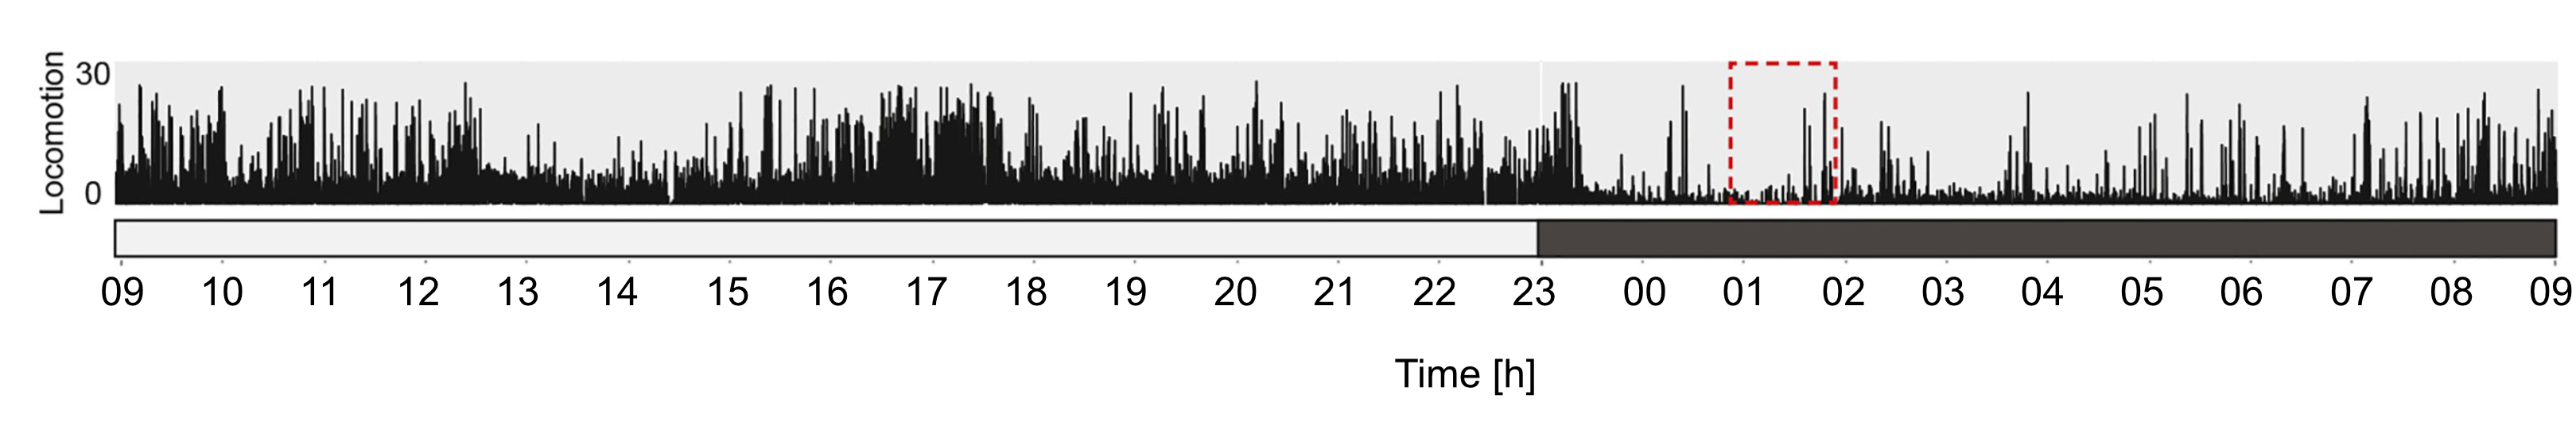
\includegraphics{zebrafish_figure_1_edited.png}
\caption{figure 1b.}
\end{figure}

\hypertarget{section-4-determining-sleep-vs-wake}{%
\subsection{Section 4: Determining sleep vs
wake}\label{section-4-determining-sleep-vs-wake}}

Distance moved over time (speed) at any given time point is used to make
calls on if a fish is asleep or awake. We can find what the cutoff they
used is by looking at what the minimum speed they call wake is and what
the maximum speed they call sleep is.

\begin{Shaded}
\begin{Highlighting}[]
\NormalTok{fish\_wake }\OtherTok{\textless{}{-}}\NormalTok{ fish\_df }\SpecialCharTok{\%\textgreater{}\%} \FunctionTok{filter}\NormalTok{(state }\SpecialCharTok{==} \StringTok{"Wake"}\NormalTok{) }
\FunctionTok{min}\NormalTok{(fish\_wake}\SpecialCharTok{$}\NormalTok{Dist\_6s)}
\end{Highlighting}
\end{Shaded}

\begin{verbatim}
## [1] 0.2000001
\end{verbatim}

\begin{Shaded}
\begin{Highlighting}[]
\NormalTok{fish\_sleep }\OtherTok{\textless{}{-}}\NormalTok{ fish\_df }\SpecialCharTok{\%\textgreater{}\%} \FunctionTok{filter}\NormalTok{(state }\SpecialCharTok{==} \StringTok{"Sleep"}\NormalTok{) }
\FunctionTok{max}\NormalTok{(fish\_sleep}\SpecialCharTok{$}\NormalTok{Dist\_6s)}
\end{Highlighting}
\end{Shaded}

\begin{verbatim}
## [1] 0.1999996
\end{verbatim}

It appears the cutoff they use is 0.2cm/s. We can see this cutoff when
we plot the raw data as well.

\begin{Shaded}
\begin{Highlighting}[]
\FunctionTok{ggplot}\NormalTok{(fish\_df, }\FunctionTok{aes}\NormalTok{(}\AttributeTok{x =}\NormalTok{ time, }\AttributeTok{y =}\NormalTok{ Dist\_6s, }\AttributeTok{colour =}\NormalTok{ state)) }\SpecialCharTok{+} \FunctionTok{geom\_line}\NormalTok{() }\SpecialCharTok{+} \FunctionTok{scale\_colour\_manual}\NormalTok{(}\AttributeTok{values =} \FunctionTok{c}\NormalTok{(}\StringTok{"lightseagreen"}\NormalTok{ , }\StringTok{"navy"}\NormalTok{)) }\SpecialCharTok{+} \FunctionTok{ggtitle}\NormalTok{(}\StringTok{"Plot 3: Zebrafish sleep vs wake speed over time"}\NormalTok{) }
\end{Highlighting}
\end{Shaded}

\includegraphics{Tutorial_2_files/figure-latex/Section 4.2-1.pdf}

And when we summarize the data with boxplots.

\begin{Shaded}
\begin{Highlighting}[]
\NormalTok{fish\_df }\SpecialCharTok{\%\textgreater{}\%} \FunctionTok{filter}\NormalTok{(day }\SpecialCharTok{==} \DecValTok{10}\NormalTok{) }\SpecialCharTok{\%\textgreater{}\%} \FunctionTok{ggplot}\NormalTok{(., }\FunctionTok{aes}\NormalTok{(}\AttributeTok{y =}\NormalTok{ Dist\_6s, }\AttributeTok{x =}\NormalTok{ state, }\AttributeTok{colour =}\NormalTok{ state)) }\SpecialCharTok{+} \FunctionTok{geom\_jitter}\NormalTok{(}\AttributeTok{alpha =} \FloatTok{0.2}\NormalTok{) }\SpecialCharTok{+} \FunctionTok{annotate}\NormalTok{(}\StringTok{"segment"}\NormalTok{, }\AttributeTok{x =} \FloatTok{0.5}\NormalTok{, }\AttributeTok{xend =} \FloatTok{2.5}\NormalTok{, }\AttributeTok{y =} \FloatTok{0.2}\NormalTok{, }\AttributeTok{yend =} \FloatTok{0.2}\NormalTok{,}\AttributeTok{linewidth =} \DecValTok{2}\NormalTok{, }\AttributeTok{colour =} \StringTok{"red"}\NormalTok{) }\SpecialCharTok{+} \FunctionTok{scale\_colour\_manual}\NormalTok{(}\AttributeTok{values =} \FunctionTok{c}\NormalTok{(}\StringTok{"lightseagreen"}\NormalTok{ , }\StringTok{"navy"}\NormalTok{)) }\SpecialCharTok{+} \FunctionTok{ggtitle}\NormalTok{(}\StringTok{"Plot 4: Zebrafish sleep vs wake cutoffs"}\NormalTok{) }
\end{Highlighting}
\end{Shaded}

\includegraphics{Tutorial_2_files/figure-latex/Section 4.3-1.pdf}

\hypertarget{section-5-sleep-timing-in-wildtype-zebrafish}{%
\subsection{Section 5: Sleep timing in wildtype
zebrafish}\label{section-5-sleep-timing-in-wildtype-zebrafish}}

Zebrafish are diurnal; when we look at the total number of observations
of sleep and wake, we can see that most sleep tends to occur during the
night and most wake occurs during the day.

\begin{Shaded}
\begin{Highlighting}[]
\FunctionTok{ggplot}\NormalTok{(fish\_WT, }\FunctionTok{aes}\NormalTok{(}\AttributeTok{x =}\NormalTok{ hour, }\AttributeTok{fill =}\NormalTok{ state)) }\SpecialCharTok{+} \FunctionTok{annotate}\NormalTok{(}\StringTok{"rect"}\NormalTok{, }\AttributeTok{xmin =} \DecValTok{0}\NormalTok{, }\AttributeTok{xmax =} \DecValTok{9}\NormalTok{, }\AttributeTok{ymin =} \DecValTok{0}\NormalTok{, }\AttributeTok{ymax =} \ConstantTok{Inf}\NormalTok{, }\AttributeTok{fill =} \StringTok{"grey"}\NormalTok{, }\AttributeTok{alpha =} \FloatTok{0.6}\NormalTok{) }\SpecialCharTok{+} \FunctionTok{annotate}\NormalTok{(}\StringTok{"rect"}\NormalTok{, }\AttributeTok{xmin =} \FloatTok{22.0}\NormalTok{, }\AttributeTok{xmax =} \FloatTok{23.9}\NormalTok{, }\AttributeTok{ymin =} \DecValTok{0}\NormalTok{, }\AttributeTok{ymax =} \ConstantTok{Inf}\NormalTok{, }\AttributeTok{fill =} \StringTok{"grey"}\NormalTok{, }\AttributeTok{alpha =} \FloatTok{0.6}\NormalTok{) }\SpecialCharTok{+} \FunctionTok{geom\_histogram}\NormalTok{(}\AttributeTok{colour =} \StringTok{"black"}\NormalTok{, }\AttributeTok{bins =} \DecValTok{25}\NormalTok{) }\SpecialCharTok{+} \FunctionTok{scale\_fill\_manual}\NormalTok{(}\AttributeTok{values =} \FunctionTok{c}\NormalTok{(}\StringTok{"slateblue4"}\NormalTok{, }\StringTok{"lightseagreen"}\NormalTok{ ))  }\SpecialCharTok{+} \FunctionTok{ggtitle}\NormalTok{(}\StringTok{"Plot 5: Total wake vs sleep observations in day vs night"}\NormalTok{)}
\end{Highlighting}
\end{Shaded}

\includegraphics{Tutorial_2_files/figure-latex/Section 5.1-1.pdf}

In wildtype zebrafish sleep is consolidated.

\begin{Shaded}
\begin{Highlighting}[]
\NormalTok{fish\_WT }\SpecialCharTok{\%\textgreater{}\%} \FunctionTok{filter}\NormalTok{(day }\SpecialCharTok{==} \DecValTok{10}\NormalTok{, hour }\SpecialCharTok{\%in\%} \DecValTok{0}\SpecialCharTok{:}\DecValTok{8}\NormalTok{) }\SpecialCharTok{\%\textgreater{}\%} \FunctionTok{ggplot}\NormalTok{(., }\FunctionTok{aes}\NormalTok{(}\AttributeTok{x =}\NormalTok{ time, }\AttributeTok{fill =}\NormalTok{ state)) }\SpecialCharTok{+} \FunctionTok{geom\_bar}\NormalTok{(}\AttributeTok{position =} \StringTok{"fill"}\NormalTok{) }\SpecialCharTok{+} \FunctionTok{scale\_fill\_manual}\NormalTok{(}\AttributeTok{values =} \FunctionTok{c}\NormalTok{(}\StringTok{"slateblue4"}\NormalTok{, }\StringTok{"lightseagreen"}\NormalTok{ )) }\SpecialCharTok{+} \FunctionTok{scale\_x\_datetime}\NormalTok{(}\AttributeTok{breaks =} \FunctionTok{date\_breaks}\NormalTok{(}\StringTok{"2 hours"}\NormalTok{))}\SpecialCharTok{+} \FunctionTok{theme}\NormalTok{(}\AttributeTok{axis.text.x =} \FunctionTok{element\_text}\NormalTok{(}\AttributeTok{angle =} \DecValTok{90}\NormalTok{))   }\SpecialCharTok{+} \FunctionTok{ggtitle}\NormalTok{(}\StringTok{"Plot 6: Zebrafish sleep"}\NormalTok{)}
\end{Highlighting}
\end{Shaded}

\includegraphics{Tutorial_2_files/figure-latex/Section 5.2-1.pdf}

\hypertarget{section-6-comparison-of-sleep-cycles-in-hypocretin-knockouts-vs-wild-type}{%
\subsection{Section 6: Comparison of sleep cycles in hypocretin
knockouts vs wild
type}\label{section-6-comparison-of-sleep-cycles-in-hypocretin-knockouts-vs-wild-type}}

Plot the comparison across all hours

\begin{Shaded}
\begin{Highlighting}[]
\NormalTok{fish\_counts }\OtherTok{\textless{}{-}}\NormalTok{ fish\_df }\SpecialCharTok{\%\textgreater{}\%} \FunctionTok{count}\NormalTok{(hour, state, genotype)}

\CommentTok{\#to get the total number of observations group by hour and genotype and then sum together all the sleep and wake observations}
\NormalTok{fish\_counts }\OtherTok{\textless{}{-}}\NormalTok{ fish\_counts }\SpecialCharTok{\%\textgreater{}\%} \FunctionTok{select}\NormalTok{(hour, state, genotype, n) }\SpecialCharTok{\%\textgreater{}\%} \FunctionTok{group\_by}\NormalTok{(hour, genotype) }\SpecialCharTok{\%\textgreater{}\%} \FunctionTok{mutate}\NormalTok{(}\AttributeTok{totals =} \FunctionTok{sum}\NormalTok{(n))}

\CommentTok{\#divide the number of sleep and wake observations by the total number of observations}
\NormalTok{fish\_counts}\SpecialCharTok{$}\NormalTok{proportions }\OtherTok{\textless{}{-}}\NormalTok{ fish\_counts}\SpecialCharTok{$}\NormalTok{n}\SpecialCharTok{/}\NormalTok{fish\_counts}\SpecialCharTok{$}\NormalTok{totals}

\NormalTok{proportion\_plot }\OtherTok{\textless{}{-}} \FunctionTok{ggplot}\NormalTok{(fish\_counts, }\FunctionTok{aes}\NormalTok{(}\AttributeTok{x =}\NormalTok{ hour, }\AttributeTok{y =}\NormalTok{ proportions, }\AttributeTok{color =}\NormalTok{ genotype)) }\SpecialCharTok{+} \FunctionTok{annotate}\NormalTok{(}\StringTok{"rect"}\NormalTok{, }\AttributeTok{xmin =} \DecValTok{0}\NormalTok{, }\AttributeTok{xmax =} \DecValTok{9}\NormalTok{, }\AttributeTok{ymin =} \DecValTok{0}\NormalTok{, }\AttributeTok{ymax =} \ConstantTok{Inf}\NormalTok{, }\AttributeTok{fill =} \StringTok{"grey"}\NormalTok{, }\AttributeTok{alpha =} \FloatTok{0.6}\NormalTok{) }\SpecialCharTok{+} \FunctionTok{annotate}\NormalTok{(}\StringTok{"rect"}\NormalTok{, }\AttributeTok{xmin =} \DecValTok{23}\NormalTok{, }\AttributeTok{xmax =} \DecValTok{24}\NormalTok{, }\AttributeTok{ymin =} \DecValTok{0}\NormalTok{, }\AttributeTok{ymax =} \ConstantTok{Inf}\NormalTok{, }\AttributeTok{fill =} \StringTok{"grey"}\NormalTok{, }\AttributeTok{alpha =} \FloatTok{0.6}\NormalTok{) }\SpecialCharTok{+} \FunctionTok{geom\_point}\NormalTok{() }\SpecialCharTok{+} \FunctionTok{geom\_line}\NormalTok{() }\SpecialCharTok{+} \FunctionTok{facet\_wrap}\NormalTok{(}\SpecialCharTok{\textasciitilde{}}\NormalTok{state) }\SpecialCharTok{+} \FunctionTok{ggtitle}\NormalTok{(}\StringTok{"Plot 7: Sleep and wake proportions in wildtype vs knockouts"}\NormalTok{)}

\NormalTok{proportion\_plot  }
\end{Highlighting}
\end{Shaded}

\includegraphics{Tutorial_2_files/figure-latex/Section 6.1-1.pdf}

\begin{figure}
\centering
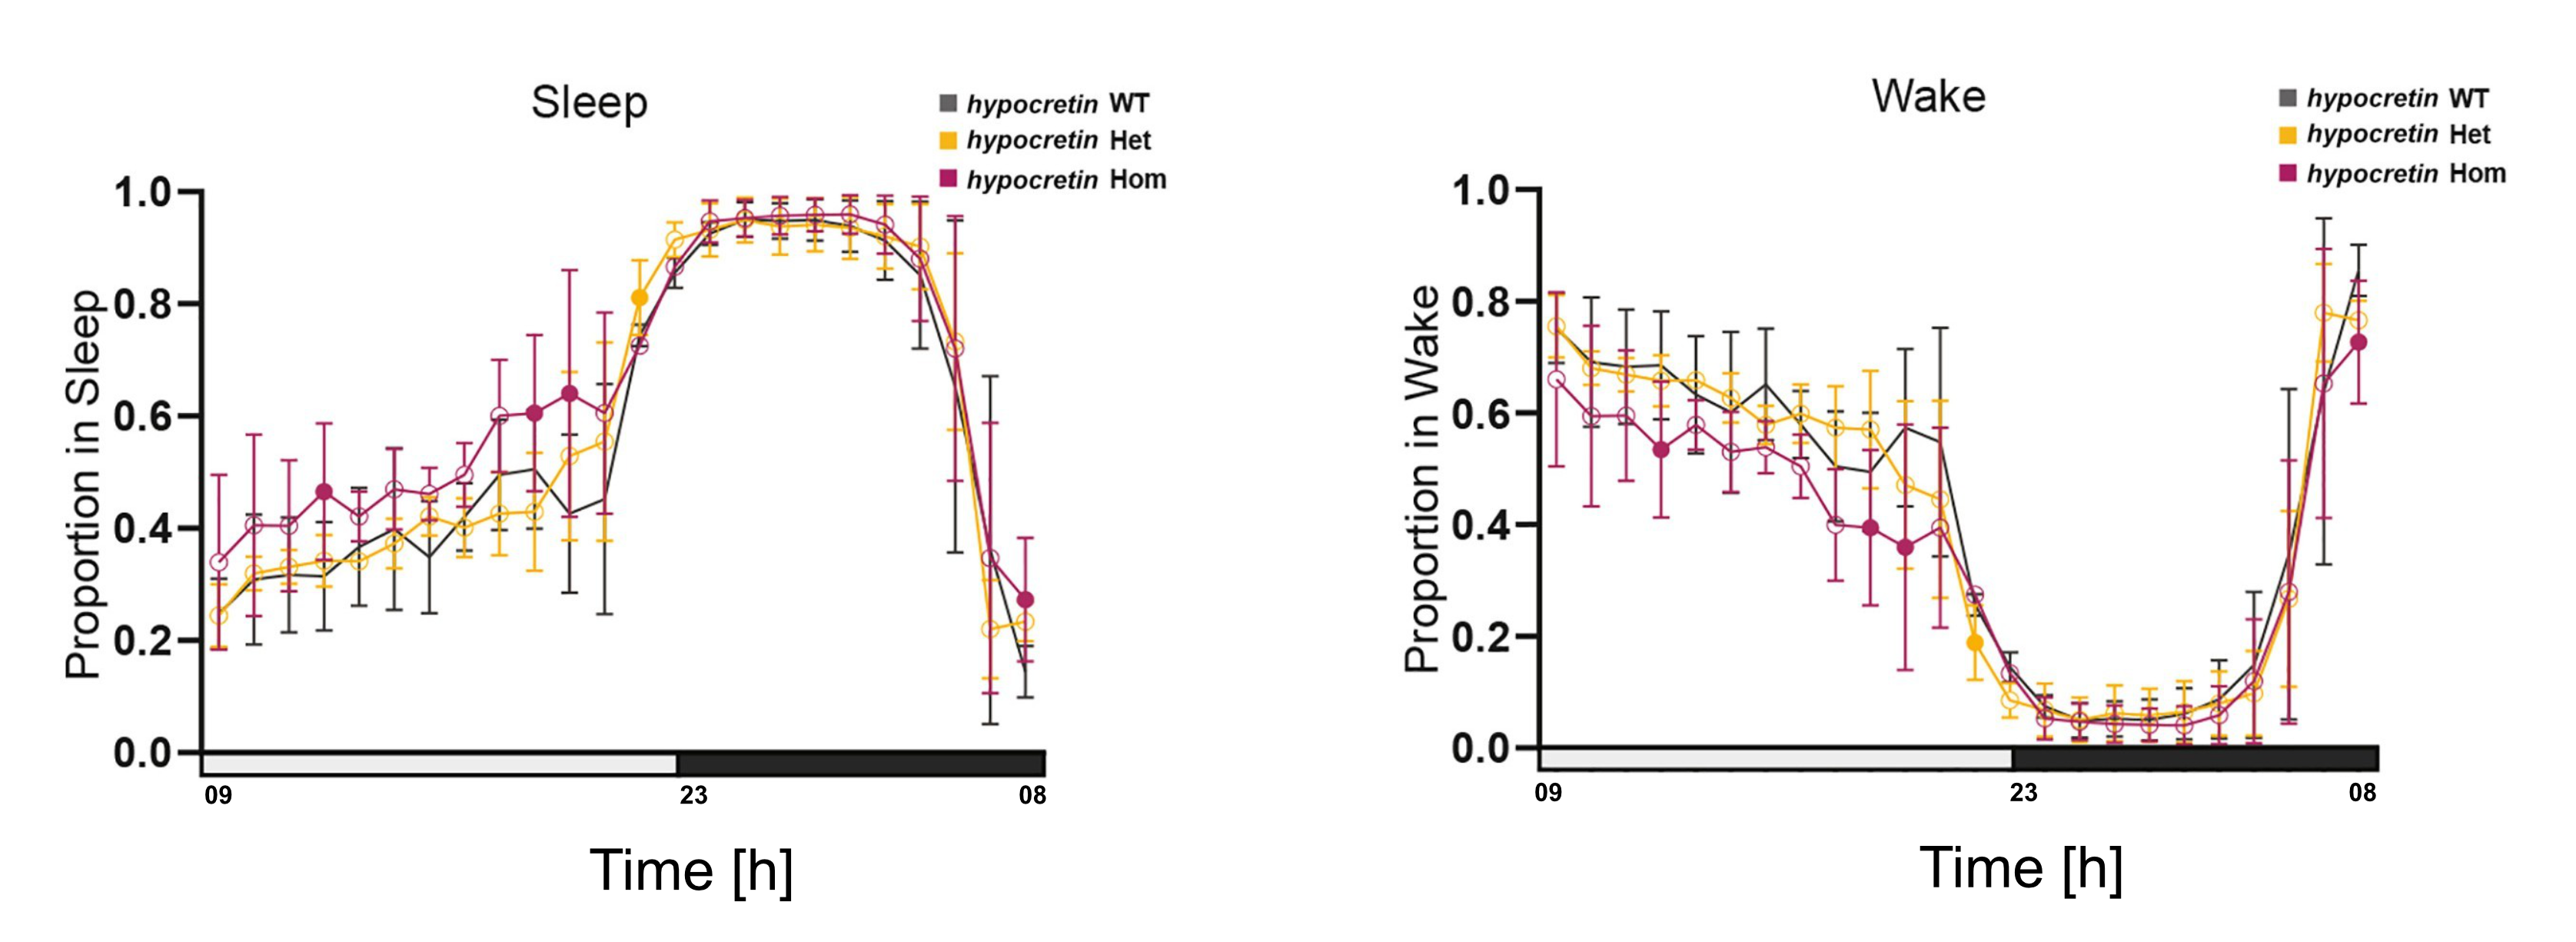
\includegraphics{zebrafish_figure_3_edited.png}
\caption{figure 1b.}
\end{figure}

Hypocretin knockout fish should have more daytime sleep than wild type.

\begin{Shaded}
\begin{Highlighting}[]
\NormalTok{fish\_counts }\SpecialCharTok{\%\textgreater{}\%} \FunctionTok{filter}\NormalTok{(hour }\SpecialCharTok{\%in\%} \DecValTok{9}\SpecialCharTok{:}\DecValTok{23}\NormalTok{, genotype }\SpecialCharTok{\%in\%} \FunctionTok{c}\NormalTok{(}\StringTok{"WT"}\NormalTok{, }\StringTok{"Hom"}\NormalTok{))  }\SpecialCharTok{\%\textgreater{}\%} \FunctionTok{ggplot}\NormalTok{(., }\FunctionTok{aes}\NormalTok{(}\AttributeTok{x =}\NormalTok{ state, }\AttributeTok{y =}\NormalTok{ n, }\AttributeTok{color =}\NormalTok{ genotype)) }\SpecialCharTok{+} \FunctionTok{geom\_boxplot}\NormalTok{() }\SpecialCharTok{+} \FunctionTok{scale\_colour\_manual}\NormalTok{(}\AttributeTok{values =} \FunctionTok{c}\NormalTok{(}\StringTok{"\#F8766D"}\NormalTok{ , }\StringTok{"\#619CFF"}\NormalTok{)) }\SpecialCharTok{+} \FunctionTok{ggtitle}\NormalTok{(}\StringTok{"Plot 8: Sleep and wake proportions in wildtype and knockouts during the day"}\NormalTok{) }
\end{Highlighting}
\end{Shaded}

\includegraphics{Tutorial_2_files/figure-latex/Section 6.2-1.pdf}

We only see this difference during the day and not during the night

\begin{Shaded}
\begin{Highlighting}[]
\NormalTok{fish\_counts }\SpecialCharTok{\%\textgreater{}\%} \FunctionTok{filter}\NormalTok{(hour }\SpecialCharTok{\%in\%} \DecValTok{0}\SpecialCharTok{:}\DecValTok{8}\NormalTok{, genotype }\SpecialCharTok{\%in\%} \FunctionTok{c}\NormalTok{(}\StringTok{"WT"}\NormalTok{, }\StringTok{"Hom"}\NormalTok{))  }\SpecialCharTok{\%\textgreater{}\%} \FunctionTok{ggplot}\NormalTok{(., }\FunctionTok{aes}\NormalTok{(}\AttributeTok{x =}\NormalTok{ state, }\AttributeTok{y =}\NormalTok{ n, }\AttributeTok{color =}\NormalTok{ genotype)) }\SpecialCharTok{+} \FunctionTok{geom\_boxplot}\NormalTok{() }\SpecialCharTok{+} \FunctionTok{scale\_colour\_manual}\NormalTok{(}\AttributeTok{values =} \FunctionTok{c}\NormalTok{(}\StringTok{"\#F8766D"}\NormalTok{ , }\StringTok{"\#619CFF"}\NormalTok{)) }\SpecialCharTok{+} \FunctionTok{ggtitle}\NormalTok{(}\StringTok{"Plot 9: Sleep and wake proportions in wildtype and knockouts during the night"}\NormalTok{)}
\end{Highlighting}
\end{Shaded}

\includegraphics{Tutorial_2_files/figure-latex/Section 6.3-1.pdf}

\begin{Shaded}
\begin{Highlighting}[]
\FunctionTok{ggplot}\NormalTok{(fish\_df, }\FunctionTok{aes}\NormalTok{(}\AttributeTok{x =}\NormalTok{ hour, }\AttributeTok{fill =}\NormalTok{ state)) }\SpecialCharTok{+} \FunctionTok{annotate}\NormalTok{(}\StringTok{"rect"}\NormalTok{, }\AttributeTok{xmin =} \DecValTok{0}\NormalTok{, }\AttributeTok{xmax =} \DecValTok{9}\NormalTok{, }\AttributeTok{ymin =} \DecValTok{0}\NormalTok{, }\AttributeTok{ymax =} \ConstantTok{Inf}\NormalTok{, }\AttributeTok{fill =} \StringTok{"grey"}\NormalTok{, }\AttributeTok{alpha =} \FloatTok{0.6}\NormalTok{) }\SpecialCharTok{+} \FunctionTok{annotate}\NormalTok{(}\StringTok{"rect"}\NormalTok{, }\AttributeTok{xmin =} \FloatTok{22.0}\NormalTok{, }\AttributeTok{xmax =} \FloatTok{23.9}\NormalTok{, }\AttributeTok{ymin =} \DecValTok{0}\NormalTok{, }\AttributeTok{ymax =} \ConstantTok{Inf}\NormalTok{, }\AttributeTok{fill =} \StringTok{"grey"}\NormalTok{, }\AttributeTok{alpha =} \FloatTok{0.6}\NormalTok{) }\SpecialCharTok{+} \FunctionTok{geom\_histogram}\NormalTok{(}\AttributeTok{colour =} \StringTok{"black"}\NormalTok{, }\AttributeTok{bins =} \DecValTok{25}\NormalTok{) }\SpecialCharTok{+} \FunctionTok{scale\_fill\_manual}\NormalTok{(}\AttributeTok{values =} \FunctionTok{c}\NormalTok{(}\StringTok{"slateblue4"}\NormalTok{, }\StringTok{"lightseagreen"}\NormalTok{ )) }\SpecialCharTok{+} \FunctionTok{facet\_wrap}\NormalTok{(}\SpecialCharTok{\textasciitilde{}}\NormalTok{genotype) }\SpecialCharTok{+} \FunctionTok{ggtitle}\NormalTok{(}\StringTok{"Plot 10: Total wake vs sleep observations in day vs night by genotype"}\NormalTok{)}
\end{Highlighting}
\end{Shaded}

\includegraphics{Tutorial_2_files/figure-latex/Section 6.4-1.pdf}

\begin{Shaded}
\begin{Highlighting}[]
\NormalTok{fish\_df }\SpecialCharTok{\%\textgreater{}\%} \FunctionTok{filter}\NormalTok{(day }\SpecialCharTok{\%in\%} \FunctionTok{c}\NormalTok{(}\DecValTok{10}\NormalTok{, }\DecValTok{14}\NormalTok{, }\DecValTok{19}\NormalTok{), hour }\SpecialCharTok{\%in\%} \DecValTok{0}\SpecialCharTok{:}\DecValTok{8}\NormalTok{) }\SpecialCharTok{\%\textgreater{}\%} \FunctionTok{ggplot}\NormalTok{(., }\FunctionTok{aes}\NormalTok{(}\AttributeTok{x =}\NormalTok{ time, }\AttributeTok{fill =}\NormalTok{ state)) }\SpecialCharTok{+} \FunctionTok{geom\_bar}\NormalTok{(}\AttributeTok{position =} \StringTok{"fill"}\NormalTok{) }\SpecialCharTok{+} \FunctionTok{scale\_fill\_manual}\NormalTok{(}\AttributeTok{values =} \FunctionTok{c}\NormalTok{(}\StringTok{"slateblue4"}\NormalTok{, }\StringTok{"lightseagreen"}\NormalTok{ )) }\SpecialCharTok{+} \FunctionTok{scale\_x\_datetime}\NormalTok{(}\AttributeTok{breaks =} \FunctionTok{date\_breaks}\NormalTok{(}\StringTok{"4 hours"}\NormalTok{)) }\SpecialCharTok{+} \FunctionTok{facet\_wrap}\NormalTok{(}\SpecialCharTok{\textasciitilde{}}\NormalTok{genotype, }\AttributeTok{ncol =} \DecValTok{1}\NormalTok{, }\AttributeTok{nrow =} \DecValTok{3}\NormalTok{, }\AttributeTok{scales =} \StringTok{"free"}\NormalTok{) }\SpecialCharTok{+} \FunctionTok{ggtitle}\NormalTok{(}\StringTok{"Plot 11: Zebrafish sleep is equally consolidated in wildtype as knockouts"}\NormalTok{)}
\end{Highlighting}
\end{Shaded}

\includegraphics{Tutorial_2_files/figure-latex/Section 6.5-1.pdf}

\end{document}
